\documentclass{beamer}% usefull options [handout]
\usepackage{graphicx}
\usepackage{wrapfig}
%\useoutertheme{infolines}
%\usetheme[height=7mm]{Rochester}
\usetheme{PaloAlto}% other nice themes Hannover, CambridgeUS, AnnArbor, Madrid, PaloAlto, Malmoe 
%\usecolortheme{dove}
%\usefonttheme{structuresmallcapsserif}
\setbeamertemplate{items}[triangle] % other options "circle", "ball", "square"
%\setbeamertemplate{blocks}[rounded][shadow=true]
%\setbeamertemplate{navigation symbols}{}

\title[Introduction to FLR]{An Introduction to FLR}
\author{FLR Core Team}

\usepackage{Sweave}
\begin{document}

\section{Introduction}

%************ Frame 1***********************
\begin{frame}[plain]
\titlepage
\end{frame}

\begin{frame}
\frametitle{Outline}
\tableofcontents[pausesections]
\end{frame}


%************ Frame 3***********************
\begin{frame}
  \frametitle{Need for FLR}

Schnute \emph{et al.} (2007 and 1998) compared the number of software tools and languages currently available for stock assessments with the Babel tower myth:
\pause\newline\newline
\textrm{{\footnotesize{
"After the people of Babel sought to build a tower to heaven, the Lord God devised a plan (Genesis 11: 4-7). 'Behold the people is one; and they all have one language; and this they began to do; and \emph{now nothing will be restrained from them, which they have imagined to do....} Let us go down, and there confound their language, that they may not understand one another's speech.' Italics highlight the prospects for accomplishment with a common language, if the scientific community could ever agree on one"
\pause\newline\newline
"The cosmic plan for \textbf{confounding software languages} seems to be working remarkably well among the community of quantitative fishery scientists!"
}}}
\end{frame}

%*********** Goals **********************
\begin{frame}
\frametitle{Goals}

To promote and generalize the use of good quality, open source, flexible software in all areas of quantitative fisheries research and management advice, with a key focus on Management Strategies Evaluation. In detail, FLR aims to facilitate and promote research about:
      \begin{itemize}
	 \item<2-> Stock assessment and provision of management advice
	 \item<3-> Data and model validation through simulation
	 \item<4-> Risk analysis
	 \item<5-> Capacity development \& education
	 \item<6-> Promote collaboration and openness in quantitative fisheries science
	 \item<7-> Support the development of new models and methods
	 \item<8-> Promote the distribution of new models and methods to a wide public.
       \end{itemize}
\end{frame}

%************ Frame 2***********************
\begin{frame}
  \frametitle{A brief history of FLR}
  
%  \begin{wrapfigure}{r}{40mm}
%	\begin{flushright}
%		
\includegraphics[width=0.20\textwidth]{flr14.jpg}
%	\end{flushright}
%  \end{wrapfigure}
  
  \begin{itemize}
	\item<1-> Started by FEMS EU project
	\item<2-> COMMIT \& EFIMAS EU projects provided much of time and sweat
	\item<3-> Presented to ICES WG Methods 2004
	\item<4-> FLCore version 1.0 - December 2005
	\begin{itemize}
		\item<4-> Release often, release early. Bugs galore
	\end{itemize}
  \end{itemize}
  \begin{itemize}
	\item<5-> FLCore version 1.4 - 2007
	\begin{itemize}
		\item<5-> Code name "The Golden Jackal"
		\item<5-> Stable, full of treats an joy
	\end{itemize}
   \end{itemize}
\end{frame}

%************ Frame 2***********************
\begin{frame}
  \frametitle{A brief history of FLR}

%  \begin{wrapfigure}{r}{40mm}
%	\begin{flushright}
%		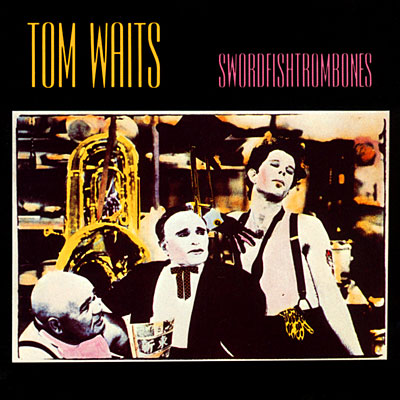
\includegraphics[width=0.20\textwidth]{flr20.jpg}
%	\end{flushright}
%  \end{wrapfigure}


  \begin{itemize}
	\item<1-> 2007-2009: The Silk Road to version 2
	\begin{itemize}
		\item<2-> New FLQuant: uncertainty in structure
		\item<2-> Rewrite of most methods
		\item<2-> Extension of methods available
		\item<2-> New classes: FLModel
		\item<2-> Stronger use of class inheritance
		\item<2-> Overhaul of man pages
		\item<2-> Simplification of package map
	\end{itemize}
  \end{itemize}
  \begin{itemize}
	\item<3-> FLCore version 2.0 - January 2009
	\begin{itemize}
		\item<3-> Code name "Swordfish Polka"
	\end{itemize}
   \end{itemize}
\end{frame}

\section{Philosophy of FLR}

%************ Frame 4***********************
\begin{frame} 
   \frametitle{Mission statement}

The FLR project provides a \textbf{platform for quantitative fisheries science} based on the R statistical language. The guiding principles of FLR are:
\begin{itemize}
	\item<2-> openness - through community involvement and the open source ethos
	\item<3-> flexibility - through a design that does not constrain the user to a given paradigm
	\item<4-> extendibility - through the provision of tools that are ready to be personalized and adapted.
\end{itemize}
\end{frame}

%************ Frame 4***********************
\begin{frame}
   \frametitle{Mission statement}

FLR's framework \textbf{facilitates and promotes collaboration} within and across disciplines, e.g. biological, ecological, statistical, mathematical, economic, and social. In particular it ensures that new modelling methods are widely available, so that alternative fisheries management strategies and procedures can be evaluated for their robustness to uncertainty before implementation.
\pause\newline\newline
FLR is distributed with an \textbf{open source} license and encourages all packages to be distributed under open source licenses in order \textbf{to promote transparency and technology transfer} between disciplines and researchers.
\end{frame}

%************ Frame 4***********************
\begin{frame}
\frametitle{Open source != free beer}
General philosophy of the open source GNU project:\newline\newline

\textrm{{\footnotesize{
"Free software is a matter of liberty, not price.  To understand the concept, one should think of \emph{free} as in \emph{free speech}, not as in \emph{free beer}."
}}}
\end{frame}

%*********** Linus **********************
\begin{frame}
\frametitle{Collaboration and Open Source}
\textrm{{\footnotesize{
"I think the real issue about adoption of open source is that nobody can really ever 'design' a complex system.  That's simply not how things work: people aren't that smart - nobody is.  And what open source allows is to not actually 'design' things, but let them evolve, through lots of different pressures in the market, and having the end result just continually improve"\newline\newline
}}}
Linus Torvalds
\end{frame}

%************ Frame 5***********************
\begin{frame}
  \frametitle{Development of FLR}
  
FLR is a collaborative development project, where distinct scientists work simultaneously on the code. This settings forced us to look for tools that were not commonly used in fisheries science, like version control systems, collaborative text writing, discussion platforms, file distribution, etc.

      \begin{itemize}
	 \item<2-> Source code is stored at R-Forge (http://r-forge.r-project.org/projects/flr/) 
	 \item<3-> Packages and tutorials etc. on wiki (http://www.flr-project.org)
	 \item<4-> Work developed under number of EU projects (FEMS, COMMIT, EFIMAS, Fisboat, UNCOVER)
	 \item<5-> Core team - maintenance and development of main packages, release official versions, test submitted packages
   \end{itemize}
\end{frame}

\section{What is FLR?}
%************ Frame 2***********************
\begin{frame}
  \frametitle{Cut the crap, what is FLR?}

FLR comprises a set of contributed packages to the open source program R. The FLR packages provide a working environment for quantitative fisheries analysis in R. 

      \begin{itemize}
	 \item<1-> Fisheries Library in R
	 \item<2-> Extendable toolbox for implementing bio-economic simulation models of fishery systems
	 \item<3-> Open source and freely available
	 \item<4-> Collaborative platform with open discussions (mailing list) and editable website
	 \item<5-> External review
	 \item<6-> Inter-disciplinary (biology, economics, social sciences)
	 \item<7-> Break barrier between user and developer
	 \item<8-> Tools used by managers as well as scientists
	 \item<9-> Many applications including:
	 \begin{itemize}
	    \item<9-> Fit stock-recruitment relationships,
	    \item<9-> Model fleet dynamics (including economics), 
	    \item<9-> Simulate and evaluate management procedures and HCRs, 
	    \item<9-> More than just stock assessment (VPA, XSA, ICES uptake)
	    \item<9-> etc....
	 \end{itemize}
   \end{itemize}

\end{frame}

\section{Design of FLR}
%************ Frame 6***********************
\begin{frame}
  \frametitle{R and FLR}
Why do we use R?
      \begin{itemize}
	 \item<2-> Existing platform for statistical modelling
	 \item<3-> Good graphics capabilities
	 \item<4-> Multi-platform
	 \item<5-> Open source
	 \item<6-> Easily extendable in the form of 'packages'
	 \item<7-> Some packages also use C / C++ code for speed (e.g. XSA) - hidden from user
      \end{itemize}
% Maybe put in that R packages figure from other beamer pres
\end{frame}

%************ Frame 7***********************
\begin{frame}
   \frametitle{Structure of FLR}
FLR uses object oriented programming
      \begin{itemize}
	 \item<2-> A programming language model organized around "objects" rather than "actions" 
	 \item<3-> Uses R S4 classes
	 \item<4-> Everything is an object of a particular class
	 \item<5-> Objects have: 
	 \begin{itemize}
	    \item<6-> members (data) and
	    \item<7-> methods (functions associated with it that act on member data)
	 \end{itemize}
	 \item<8-> Inheritence used to extend and create new classes (FLSR inherits from FLModel)
	 \item<9-> Classes can be members of other classes (most FLR classes include FLQuants as members)
      \end{itemize}
\end{frame}

%************ Frame 7***********************
\begin{frame}
   \frametitle{Structure of FLR - Design principles}
      \begin{itemize}
	 \item<2-> Classes to represent different elements of fisheries systems
	 \item<3-> 'physical' objects (e.g. FLStock class represents a fish stock)
	 \item<4-> 'methodological' objects (e.g. FLBRP class containing methods to calculate BRP)
	 \item<5-> Link objects to create simulations - Lego blocks (MSE example)
	 \item<6-> Learning curve: trade off between flexibility and simplicity (no black boxes and no handle turning)
      \end{itemize}
\end{frame}

%************ Frame 8***********************
\begin{frame}
  \frametitle{MSE - The Lego block approach}
   \begin{center}
      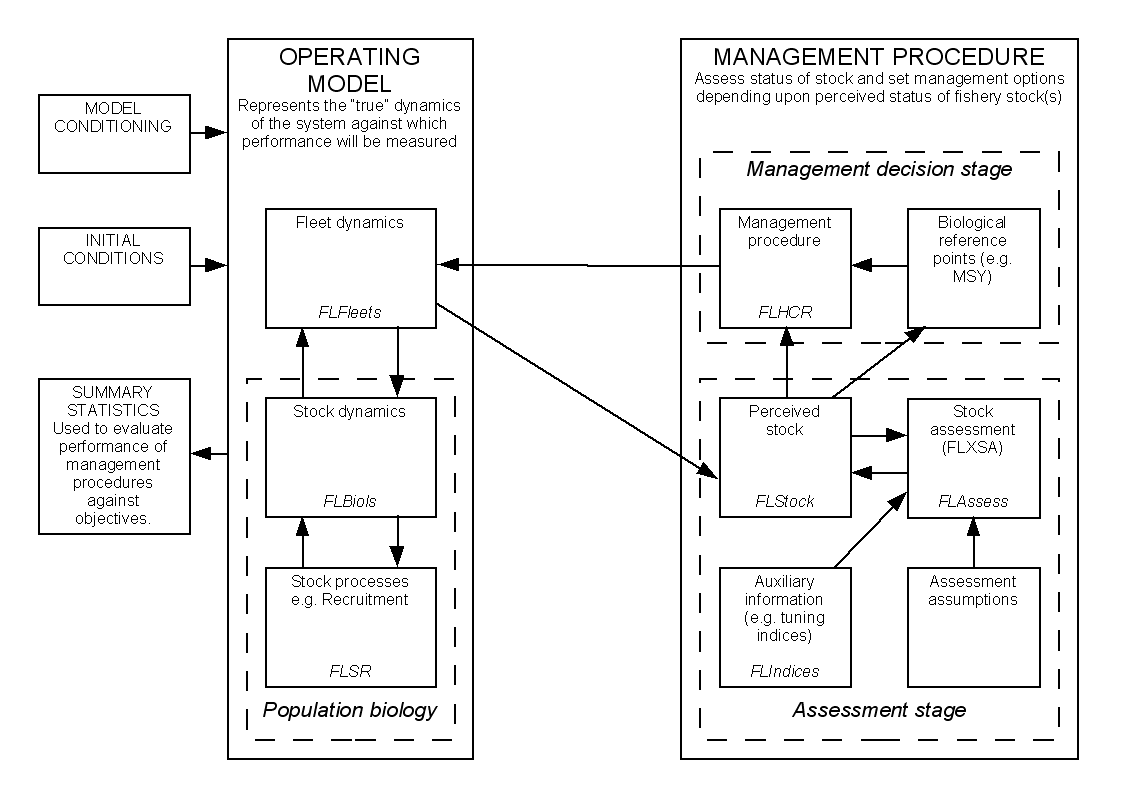
\includegraphics[width=0.8\textwidth]{MSE.png}
   \end{center}
\end{frame}

%*********** Frame ***********************
%\begin{frame}
%   \frametitle{What's in a package?}
%      \begin{itemize}
%	 \item<2-> R code (and C code) for classes, methods and functions
%	 \item<3-> Help pages
%	 \item<4-> Examples
%	 \item<5-> Data sets
%	 \item<6-> Test scripts.
%      \end{itemize}
%\end{frame}

\section{What's next ?}
%*********** Frame ***********************
\begin{frame}
   \frametitle{What's next ?}
	\begin{center}
		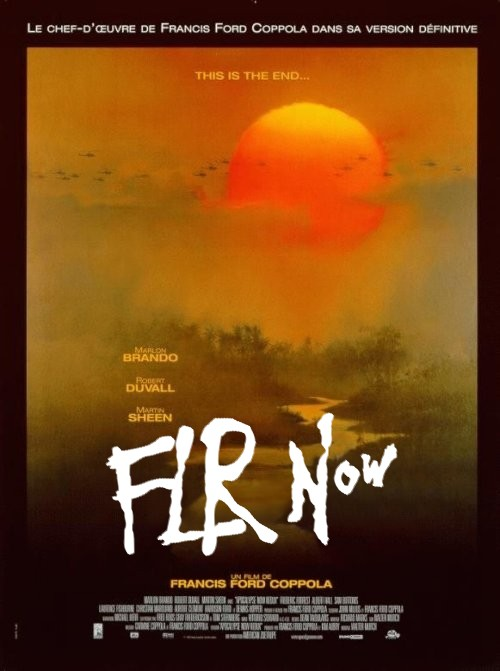
\includegraphics[width=0.45\textwidth]{flr30.jpg}
	\end{center}
\end{frame}

\end{document}
